%%%%%%%%%%%%%%%%%%%%%%%%%%%%%%%%%%%%%%%%%%%%%%%%%%%%%%%%%%%%%%%%%%%%
%% I, the copyright holder of this work, release this work into the
%% public domain. This applies worldwide. In some countries this may
%% not be legally possible; if so: I grant anyone the right to use
%% this work for any purpose, without any conditions, unless such
%% conditions are required by law.
%%%%%%%%%%%%%%%%%%%%%%%%%%%%%%%%%%%%%%%%%%%%%%%%%%%%%%%%%%%%%%%%%%%%

\documentclass[
  digital, %% The `digital` option enables the default options for the
           %% digital version of a document. Replace with `printed`
           %% to enable the default options for the printed version
           %% of a document.
%%  color,   %% Uncomment these lines (by removing the %% at the
%%           %% beginning) to use color in the digital version of your
%%           %% document
  table,   %% The `table` option causes the coloring of tables.
           %% Replace with `notable` to restore plain LaTeX tables.
  twoside, %% The `twoside` option enables double-sided typesetting.
           %% Use at least 120 g/m² paper to prevent show-through.
           %% Replace with `oneside` to use one-sided typesetting;
           %% use only if you don’t have access to a double-sided
           %% printer, or if one-sided typesetting is a formal
           %% requirement at your faculty.
  lof,     %% The `lof` option prints the List of Figures. Replace
           %% with `nolof` to hide the List of Figures.
  lot,     %% The `lot` option prints the List of Tables. Replace
           %% with `nolot` to hide the List of Tables.
  %% More options are listed in the user guide at
  %% <http://mirrors.ctan.org/macros/latex/contrib/fithesis/guide/mu/fi.pdf>.
]{fithesis3}
%% The following section sets up the locales used in the thesis.
\usepackage[resetfonts]{cmap} %% We need to load the T2A font encoding
\usepackage[T1,T2A]{fontenc}  %% to use the Cyrillic fonts with Russian texts.
\usepackage[
  main=english, %% By using `czech` or `slovak` as the main locale
                %% instead of `english`, you can typeset the thesis
                %% in either Czech or Slovak, respectively.
  english, german, russian, czech, slovak %% The additional keys allow
]{babel}        %% foreign texts to be typeset as follows:
%%
%%   \begin{otherlanguage}{german}  ... \end{otherlanguage}
%%   \begin{otherlanguage}{russian} ... \end{otherlanguage}
%%   \begin{otherlanguage}{czech}   ... \end{otherlanguage}
%%   \begin{otherlanguage}{slovak}  ... \end{otherlanguage}
%%
%% For non-Latin scripts, it may be necessary to load additional
%% fonts:
\usepackage{paratype}
\def\textrussian#1{{\usefont{T2A}{PTSerif-TLF}{m}{rm}#1}}
%%
%% The following section sets up the metadata of the thesis.
\thesissetup{
    date        = \the\year/\the\month/\the\day,
    university  = mu,
    faculty     = fi,
    type        = bc,
    author      = Jane Doe,
    gender      = f,
    advisor     = {Prof. RNDr. John Smith, CSc.},
    title       = {The Proof of P = NP},
    TeXtitle    = {The Proof of $\mathsf{P}=\mathsf{NP}$},
    keywords    = {keyword1, keyword2, ...},
    TeXkeywords = {keyword1, keyword2, \ldots},
    abstract    = {%
      This is the abstract of my thesis, which can

      span multiple paragraphs.
    },
    thanks      = {%
      These are the acknowledgements for my thesis, which can

      span multiple paragraphs.
    },
    bib         = example.bib,
    %% Uncomment the following line (by removing the %% at the
    %% beginning) and replace `assignment.pdf` with the filename
    %% of your scanned thesis assignment.
%%    assignment         = assignment.pdf,
}
\usepackage{makeidx}      %% The `makeidx` package contains
\makeindex                %% helper commands for index typesetting.
%% These additional packages are used within the document:
\usepackage{paralist} %% Compact list environments
\usepackage{amsmath}  %% Mathematics
\usepackage{amsthm}
\usepackage{amsfonts}
\usepackage{url}      %% Hyperlinks
% \usepackage{markdown} %% Lightweight markup
\usepackage{tabularx} %% Tables
\usepackage{tabu}
\usepackage{booktabs}
\usepackage{listings} %% Source code highlighting
\lstset{
  basicstyle      = \ttfamily,
  identifierstyle = \color{black},
  keywordstyle    = \color{blue},
  keywordstyle    = {[2]\color{cyan}},
  keywordstyle    = {[3]\color{olive}},
  stringstyle     = \color{teal},
  commentstyle    = \itshape\color{magenta},
  breaklines      = true,
}
\usepackage{floatrow} %% Putting captions above tables


% \usepackage{threeparttable}
% \usepackage{lscape}

\floatsetup[table]{capposition=top}
\begin{document}

\chapter*{Introduction}
\addcontentsline{toc}{chapter}{Introduction}

This thesis was developed in collaboration with \emph{Red Hat}\footnote{See \url{https://www.redhat.com/en}} as a research project.
Partners from \emph{Red Hat} provided expert guidance throughout the whole process of the thesis development and infrastructure for the dataset gathering and model training.
% todo
(Mal by v uvode byt tento odstavec? Ak ano tak kde?)

Open source software (OSS) is a type of computer software in which source code is released under a license in which the copyright holder grants users the rights to use, study, change, and distribute the software to anyone and for any purpose\footnote{See \url{https://books.google.cz/books?id=04jG7TTLujoC&pg=PA4&redir_esc=y\#v=onepage&q&f=false}}.
Open source projects have an increasing relevance in modern software development.
For example, many critical software systems are currently available under open source licenses, including operating systems, compilers, databases, and web servers.
Similarly, it is common nowadays to depend on open source libraries and frameworks when building and evolving proprietary software \cite{p:7}.

\emph{GitHub}\footnote{See \url{https://github.com/}} is the world’s largest collection of open source software, with more than 56 million users and 100 million projects.
It offers the distributed version control and source code management functionality of \emph{Git}\footnote{See \url{https://git-scm.com/}} and some more features.

\subsection*{Aim}

As more and more technologies rely on open source software, it is important to put a lot of attention into choosing such dependencies.
If an open source repository ceases to be actively developed and becomes obsolete, it can cause serious issues for all of the other projects that depend on this repository.
It would be helpful to be able to determine if a \emph{GitHub} hosted repository has a high chance of being actively developed in the future, or if it will likely die off.
The aim of this thesis is precisely that, to develop a \emph{machine learning}\footnote{See \url{https://en.wikipedia.org/wiki/Machine_learning}} model to estimate a probability of survival of \emph{GitHub} repositories.

\subsection*{Key contributions}

I developed applications \ref{sec:applications} for gathering relevant data that can be used to construct an input dataset for \emph{machine learning} models \ref{sec:training_evaluation}.
I also proposed and tested a set of features \ref{chap-2:features} for determining project's survivability.

\subsection*{Contents}

Chapter \ref{chap-1:review} goes over some research papers aiming to solve a similar problem as this thesis.
In the chapter \ref{chap-2:features}, I go over proposed features and give an explanation of what they measure and why I decided to include them.
Chapter \ref{chap-3:implementation} describes the process of gathering and preparing data, as well as methods used for training and evaluating machine learning models used for making predictions.
Then, the chapter \ref{chap-4:results} provides a summary and analysis of the achieved results.
The final chapter, chapter \ref{chap-5:summary}, provides a summary of the thesis.



\chapter{Previous work}
\label{chap-1:review}
% 8 -> unmaintained projects -> last commit from more than a year ago
% 7, 8, 9, 12, 17, ...

% nenasiel som ziaden papier co by sa pokusal robit to co robim ja
% ja tiez, ako aj ine papiere, na klasifikovanie pouzivam pevne, mnou dane pravidla
% ale ja sa pomocou ai snazim zistit ci budu maintained porjekty v buducnosti unmaintained
% co teda opisovat v "previous work"?

There already are several research papers classifying projects as maintained or unmaintained.
% todo pridat citacie na papiere
These papers, however, 
This chapter goes through them, analyses problems they are trying to solve, methods they use and results they obtained.

\section{Papers}

\subsection{Identifying Unmaintained Projects in GitHub}
\label{temp:paper1}

\subsubsection{Introduction}

\citeauthor{p:7} proposed an approach to identify GitHub projects that are not actively maintained.
Their goal is to detect unmaintained repositories as soon as possible.
The definition of unmaintained is different from the definition used in this project \ref{sec:filtering}.
% todo dopisat v com sa tie 2 definicie lisia - str 2 - 1. odstavec

Ten models were trained for the identification.
The best model was then validated by means of survey with the owners of projects classified as unmaintained.

\subsubsection{Dataset}

Initial dataset was the top 10 000 most starred repositories on GitHub.
Three strategies were used to filter out not suitable repositories:

\begin{enumerate}
    \item Remove repositories with less than 2 years between the first and the last commit.
    Models need historical data.
    2 810 repositories were removed this way.

    \item Remove repositories with null size, measured in lines of code.
    Typically projects implemented in non-programming languages.
    331 repositories were removed.

    \item Remove 74 non-software repositories.
    These are identified by searching for the topics \emph{books} and \emph{awesome-lists}.
\end{enumerate}

Stripped down version of the original dataset contains 6785 repositories.
In the next step in data preparation process, 1 002 repositories were selected from the filtered dataset and split into two categories.

\begin{enumerate}
    \item Active: 754 projects that have at least one release in the last month.

    \item Unmaintained: 248 projects that were either: (1) explicitly declared as unmaintained by their principal developers or (2) archived.
\end{enumerate}

\subsubsection{Features}

Figure \ref{fig:p7-features} lists used features.
These features do not refer to the whole history of the project, but only to the last \emph{n} months, counting from the last commit.
Each feature were collected in the interval of \emph{m} months.
Authors experimented with different combinations of \emph{n} and \emph{m} called scenarios.
For each scenario, they used a clustering analysis to remove correlated features.

\begin{figure}
    \centering
    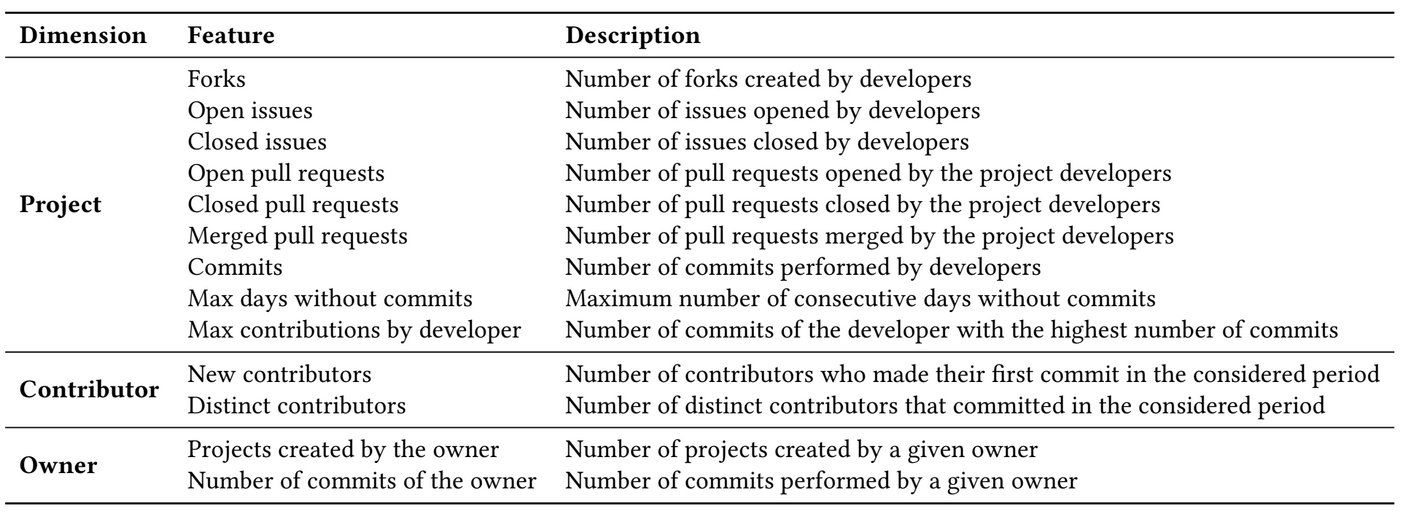
\includegraphics[scale=0.3]{chapters/chapter1/p7-features.png}
    \caption{Features \cite{p:7}}
    \label{fig:p7-features}
\end{figure}

\subsubsection{Models}

Out of ten tested models, Random Forest achieved the best results.
Two baselines were compared: \#1 all projects are predicted as unmaintained and \#2 random predictions.
Models were validated using a 5-fold cross validation.
Six metrics were used to evaluate a performance of classifier:

\begin{enumerate}
    \item precision
    \item recall
    \item F-measure
    \item accuracy
    \item AUC
    \item Kappa
\end{enumerate}

\subsubsection{Results}

The best results -- a precision of 80\% and a recall of 96\% -- were achieved when features were collected for the time period of 2 years in interval of 3 months.
Random Forest also produces a measure of the importance of the features.
The most important features are:

\begin{enumerate}
    \item number of commits
    \item maximal number of days without commits 
    \item maximal contributions by a developer
    \item number of closed issues
\end{enumerate}


\chapter{Features}
\label{chap-2:features}

\begin{table}
  \begin{tabular}{|c|}
    \toprule
    Features \\
    \midrule
    pulls\_count\_open \\
    pulls\_count\_closed \\
    issues\_count\_open \\
    issues\_count\_closed \\
    commits\_count \\
    branches\_count \\
    releases\_count \\
    owner\_type \\
    watchers\_count \\
    forks\_count \\
    stargazers\_count \\
    development\_time \\
    owner\_account\_age \\
    avg\_dev\_account\_age \\
    has\_test \\
    has\_doc \\
    has\_example \\
    has\_readme \\
    owner\_projects\_count \\
    owner\_following \\
    owner\_followers \\
    devs\_followers\_avg \\
    devs\_following\_avg \\
    commits\_by\_dev\_with\_most\_commits \\
    magnetism \\
    stickiness \\
    wealth \\
    last\_commit\_age \\
    \bottomrule
  \end{tabular}
  \caption{Features}
  \label{tab:features}
\end{table}

GitHub repositories are analyzed based on seven different areas.
Each area considers a different aspect of a repository.
Similar works (todo pridat citacie na papiere) analyze repositories in only one extent.
I combined them and gave models (referencia na modely) an overview of a repository qualities across several dimensions. 

The idea is that a repository that is lacking in some of the areas can still excel in others.
Higher number of analyzed features from different categories might result in a better accuracy of classification models.
Some of the models will be able to determine which feature area is better for estimating project survivability than others.
This information might help project owners and contributors to figure out which area their project they should improve on, to increase the chances of a project survival.

These areas and their corresponding sections are:

\begin{itemize}
    \item Popularity \ref{sec:popularity}
    \item Community growth \ref{sec:comm_growth}
    \item Community activity \ref{sec:comm_activity}
    \item Management (zmenit) \ref{sec:management}
    \item Maintenance \ref{sec:maintenance}
    \item Maturity (zmenit) \ref{sec:maturity}
    \item Development rate \ref{sec:development_rate}
\end{itemize}

List of features can be seen in the table \ref{tab:features}.
All of these features are fed as an input for the learning algorithms, they are grouped into areas for the better understandability.

\section{Popularity}
\label{sec:popularity}

Features measured in this category:

\begin{itemize}
    \item stargazers\_count: number of stars
    \item watchers\_count: number of watchers
    \item forks\_count: number of forks
\end{itemize}

While not stated explicitly by GitHub, number of stars\footnote{See \url{https://docs.github.com/en/enterprise-server@2.22/github/getting-started-with-github/github-glossary\#star}} and watchers\footnote{See \url{https://docs.github.com/en/github/getting-started-with-github/be-social\#watching-a-repository}} can be considered as a measure of a project's popularity.

GitHub \emph{stars} are intended to be used primarily to bookmark a repository\footnote{See \url{https://docs.github.com/en/github/getting-started-with-github/saving-repositories-with-stars}}.
Users can also use it as a form of appreciation for the project, it is often used as a proxy for a project popularity \cite{p:1} \cite{p:2} \cite{p:3} \cite{p:6}, even by GitHub\footnote{See \url{https://github.com/trending}}.
Because of ambiguity in terms of user's intentions to \emph{star} a project, I do not consider sufficient to use it as the only popularity metric.

To \emph{watch} a repository, means that the user is interested in getting notified on changes in that repository.
This can indicate a stronger interest than a \emph{star}, as user will receive information about changes in the repository.

Repository might be \emph{forked} when a developer intends to contribute to submit pull requests, fix bugs, add new features and keep copies etc.
These might not be the only reasons to fork a repository, however, high number of forks can still show a high popularity.
Developers are also more likely to fork a project in their preferred programming language \cite{p:10}.

\section{Community growth}
\label{sec:comm_growth}

Features measured in this category:

\begin{itemize}
    \item magnetism
    \item stickiness
\end{itemize}

Magnet projects are those that \textbf{attract a large proportion of new contributors}.
\emph{Magnetism} of a project is the proportion of contributors who made their first contribution in the time period under study who contribute to a given project \cite{p:11}.

In this project, magnetism is computed as a quotient of a number of \emph{new} contributors and a number of \emph{old} contributors.
Old contributors are contributors who committed to the project before a time threshold of two years.
% treba nejak dalej rozvyt tie 2 roky? ze napr. 2 roky pred aktualnym datumom? to by potom trebalo niekde napisat aky je aktualny datum
New contributors, on the other hand, are contributors who committed to the project only after the time threshold.

Figure \ref{fig:magnetism} shows the difference between \emph{new} and \emph{old} contributors, T represents time of the study and A represents time two years before the study.
Developers that contributed to the project before A, the red line, are considered \emph{old} contributors.
Developers that contributed to the project after A, the blue line, are considered \emph{new} contributors.

\begin{figure}
    \centering
    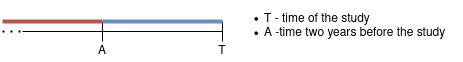
\includegraphics[scale=0.75]{chapters/chapter2/magnetism-new.png}
    \caption{Magnetism}
    \label{fig:magnetism}
\end{figure}

Sticky projects are those where a large proportion of the contributors will keep making contributions in the time period the following and under study \cite{p:11}.
Stickiness in this project is calculated as a quotient of number of contributors that \emph{sticked} and a number of \emph{new} contributors.
Contributors are considered \emph{New} if they commit to the project within past two years.
Contributors that \emph{sticked} are those \emph{new} contributors who still committed to the project within the past year.
It is the proportion of contributors who worked on a given project in the period between one to two years before the study, who also continued to make contributions for the past year before the study.

Figure \ref{fig:stickiness} shows the difference between \emph{new} and \emph{sticked} contributors, T represents time of the study, B represents time two years before the study and A represents time one year before the study.
Developers that contributed to the project between B and A, the red line, are considered \emph{new} contributors.
Developers that contributed to the project between A and T, the blue line, are considered \emph{sticked} contributors.

\begin{figure}
    \centering
    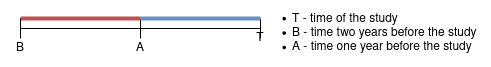
\includegraphics[scale=0.75]{chapters/chapter2/stickiness-new.png}
    \caption{Stickiness}
    \label{fig:stickiness}
\end{figure}

While magnetism metric can indicate how good the project is at attracting new contributors, stickiness can show how good the project is at keeping the new contributors.

\section{Community activity}
\label{sec:comm_activity}

Features measured in this category:

\begin{itemize}
    \item commits\_by\_dev\_with\_most\_commits: number of commits by a contributor with the highest number of commits
    \item devs\_followers\_avg: average number of a repository contributor's followers
    \item devs\_following\_avg: average number of repositories followed by a repository contributor's
\end{itemize}

Small minority of the most active project contributors tend to produce the most activity \cite{top_dev}.
For this reason, it might be useful to consider the most active contributor.
This can be done in several ways.
Measures of activity can be frequency of commits, code addition in commits, message frequency in \emph{Pull requests}\footnote{See \url{https://docs.github.com/en/enterprise-server@2.22/github/getting-started-with-github/github-glossary\#pull-request}} and \emph{Issues}\footnote{See \url{https://docs.github.com/en/enterprise-server@2.22/github/getting-started-with-github/github-glossary\#issue}} and others.
In this project, the most active contributor is selected based on the number of commits.

The average number of followers of developers in the project and the average number of developers/projects followed by them can be seen as an approximation of social relations of project members.
It turns out that project whose developers follow many others are in general more popular.
The effect for developers being followed by many others (i.e. having popular developers in the project) is much weaker.
This discovery results in a practical advice for projects: finding developers engaged in the community is good for the project popularity and can be measured by a simple proxy quantity \cite{p:14}.
Having more popular contributors might improve the project's longevity.

Initially, there was supposed to be another feature in this area, \emph{health}.
In terms of OSS, it is defined as a indicative of three factors of how community activities are performed in a project:

\begin{itemize}
    \item workrate of each contributor
    \item attractiveness of new contributors to a community
    \item active retention of experienced members
\end{itemize}

Labor is measured as community contributions within the projects.
Only source code changes as contributions are considered (i.e., comments made by contributors are ignored) \cite{p:18}.

Although this metric is interesting and potentially very insightful, its computation requires a considerable amount of GitHub API calls\footnote{See \url{https://docs.github.com/en/rest}} to which I have a limited access to.
Compared to most of the other features, it is also resource heavy, which is not suitable for the project of this scale.
For these reasons, I decided to drop this feature, it could be added in the future work.

\section{Management}
\label{sec:management}

Features measured in this category:

\begin{itemize}
    \item owner\_type: type of the repository owner, can be either \emph{organization} or \emph{personal}
    \item owner\_projects\_count: number of repository owner's repositories
    \item owner\_following: number of repositories that the repository owner follows
\end{itemize}

GitHub offers two types of accounts\footnote{See \url{https://docs.github.com/en/github/getting-started-with-github/types-of-github-accounts}}: \emph{personal} and \emph{organization}.
Personal accounts are intended for individual users while organization accounts are for groups of people to collaborate across many projects at once.
Developers are more likely to fork a repository owned by an \emph{organization} type owner \cite{p:10}.

Rationale for the number of project owner's other projects is that the the high number of them might negatively affect the level of maintenance each of them get \cite{p:7}.

Number of repositories followed by the project's owner, the out-degree, tends to be linked with more forks of the project \cite{p:10}.

\section{Maintenance}
\label{sec:maintenance}

Features measured in this category:

\begin{itemize}
    \item has\_test: whether a repository contains a dedicated test code
    \item has\_doc: whether a repository contains a documentation
    \item has\_readme: whether a repository contains a README file
    \item has\_example: whether a repository contains an usage examples
    \item issues\_count\_open: number of \emph{open} issues
    \item issues\_count\_closed: number of \emph{closed} issues
\end{itemize}

Test folder provides the test code for quality assurance, and may help others to test the code they contribute \cite{p:4}.
This makes contributing easier and thus may attract new developers.
Tests are often run periodically in an automated fashion as a part of CI/CD workflow\footnote{See \url{https://www.redhat.com/en/topics/devops/what-is-ci-cd}}.
Such practice greatly improves bug detection and can improve overall project quality.
% todo mozno napisat ze preco tieto stringy?
In this project, a file is considered a test file if it is in a folder named "test, "tests, "t" or "spec".
Presence of a dedicated test folder\footnote{Example \url{https://github.com/jekyll/jekyll}} is shown to be positively correlated with increased number of project forks \cite{p:4}.

It is shown that presence of a proper project documentation is positively associated with the usability improvement of an OSS project \cite{documentation}.
Proper documentation increases understandability and learn-ability of a software.
In this way, it may help with the project maintenance, as new developers are able to join existing community more smoothly.
Project documentation can be provided in several ways.
For smaller projects, it might be sufficient to cover all of the documentation in the \emph{README} file.
Larger projects often require several dedicated documents.
These documents might be incorporated into the GitHub repository\footnote{Example \url{https://github.com/electron/electron}}, or they can reside outside of the repository, for example on the project's web page\footnote{Example \url{https://github.com/facebook/react}}.
Detecting a documentation living outside of the repository would be difficult to do in an automated manner.
% todo mozno dopisat ako som dosiel k tym stringom ktore hladam - vycital som to z papiera 4
This feature looks for a directory named \emph{doc}, \emph{docs}, \emph{document} or \emph{documents}.

As mentioned above, \emph{README}\footnote{See \url{https://docs.github.com/en/github/creating-cloning-and-archiving-repositories/about-readmes}} file may contain a project's documentation.
That is usually the case for very small projects.
It is typically the first thing an user sees in the repository and generally contains information about what the project does, who are its intended users, use cases and so on.
Detecting a \emph{README} file is a straight forward process, we look for a file named \emph{README} in any case and with any extension.

Projects may contain an \emph{examples} folder, containing various usage examples\footnote{Example \url{https://github.com/kubernetes/client-go}}.
Presence of an examples folder may indicate the desire to attract an external attention \cite{p:4}, as these examples are helpful especially for the new users.
In terms of this project, detecting an \emph{examples} folder means searching for the folder named either \emph{example} or \emph{examples}.

The use of these folders suggests a practice of following conventional folder structure in these projects \cite{p:4}.

\emph{GitHub issues}\footnote{See \url{https://docs.github.com/en/enterprise-server@2.20/github/getting-started-with-github/github-glossary\#issue}} can be used for bug reporting, requesting features\footnote{See \url{https://guides.github.com/features/issues/}}, and others.
Creating and commenting on an issue is one of the forms of communication between users of the project and its developers.
It is also often a starting point for new contributors, especially issues labeled as \emph{good first issues} \cite{newcomers}.
Amount of open and closed issues might be a good indicator of two things: project's usage and level of involvement of the developer team.

\section{Maturity}
\label{sec:maturity}

Features measured in this category:

\begin{itemize}
    \item development\_time: time between the first and the latest commit
    \item avg\_dev\_account\_age: average of a repository contributor's accounts age in days
    \item owner\_account\_age: age of repository owner's account in days
    \item owner\_followers: number of a repository owner followers
\end{itemize}

Repository \emph{development time} \label{feature:development_time} is measured in days.
The rationale: projects that are being developed over longer periods of time and are still active have also higher chance of continuing to be active in the future.
It is also an important feature separate suitable repositories for this study from the rest.
Because of many features that require historical data, only projects developed for more than 730 days are being considered.

Note that time between the first and the last commit is not necessarily the same thing as the repository age.
Difference can be demonstrated on the example: repository illustrated in the figure \ref{fig:repo_age} was being actively developed for less than a year.
Other repository, illustrated in the figure \ref{fig:development_age} was being actively developed for almost 2 years, the most recent commit added not very long ago.
Red line in the figures represents development of the project.
Ages of both of these repositories are two years, however, second repository \ref{fig:development_age} clearly has a higher chance of continuing to being actively developed, than the first one \ref{fig:repo_age}.

\begin{figure}
    \centering
    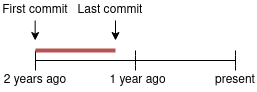
\includegraphics[scale=0.75]{chapters/chapter2/repo_age.png}
    \caption{Shorter development time}
    \label{fig:repo_age}
\end{figure}

\begin{figure}
    \centering
    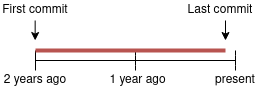
\includegraphics[scale=0.75]{chapters/chapter2/development_age.png}
    \caption{Longer development time}
    \label{fig:development_age}
\end{figure}

Having newer developers in the project is positively correlated with its popularity.
This phenomenon can probably be explained by the fact that programmers may join GitHub in order to contribute to attractive projects \cite{p:14}.
As mentioned in the section \ref{sec:popularity}, gain in popularity can attribute to the project's longevity.

More popular repository owners tend to have older GitHub accounts \cite{p:10}.
Popularity in this context means that repositories of these owners are being forked more often.
Reason for this may be that older project owners (project owners with older GitHub account) are more established in the community or own more projects that are potentially successful.

Related to project owner's popularity is also a number of owner's followers.
More popular owners usually have more followers \cite{p:14}.

\section{Development rate}
\label{sec:development_rate}

Features measured in this category:

\begin{itemize}
    \item commits\_count: number of commits
    \item pulls\_count\_open: number of \emph{open} pull requests
    \item pulls\_count\_closed: number of \emph{closed} pull requests
    \item branches\_count: number of branches
    \item releases\_count: number of releases
    \item wealth: weighted measure based on Pull Requests
    \item last\_commit\_age: age of the last commit in days
\end{itemize}

Features \emph{number of commits}, \emph{number of open pull requests}, \emph{number of branches} and \emph{age of the last commit} are closely related.
To better understand their importance for the study it will be helpful to explain the standard workflow of contribution to a GitHub repository.

\begin{figure}
    \centering
    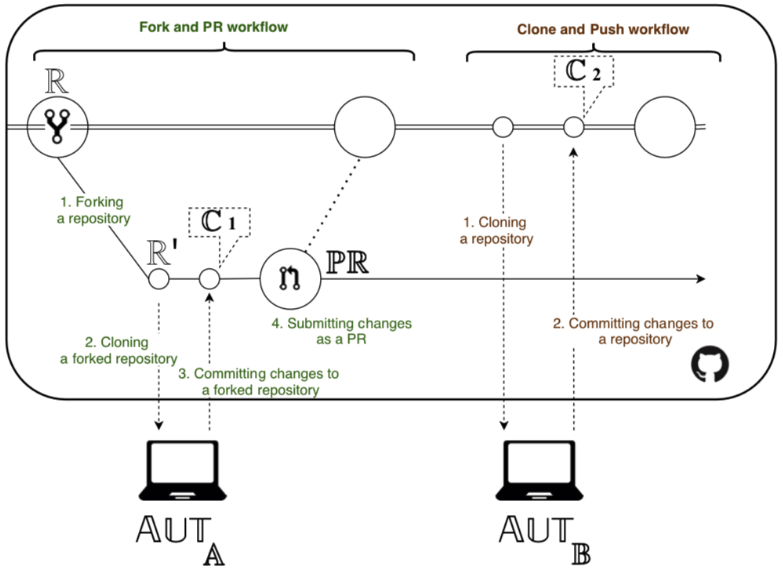
\includegraphics[scale=0.5]{chapters/chapter2/git_workflow.png}
    \caption{Scheme of two types of GitHub workflows \cite{git_workflow}}
    \label{fig:git_workflow}
\end{figure}

Figure \ref{fig:git_workflow} illustrates two types of GitHub contribution workflows: a) Fork and PR workflow and b) Clone and Push workflow.

% todo treba aj toto citovat?
$\mathbb{R}$ denotes a repository, $\mathbb{C}$ set of commit changes and $\mathbb{PR}$ represents a pull request \cite{git_workflow}.

\subsection{Fork and Pull Request (PR) workflow}
\label{sec:fork_pr}

\begin{enumerate}
    \item Fork a repository: A fork is a copy of a repository.
    Forking a repository allows user to freely experiment with changes without affecting the original project.
    Most commonly, forks are used to either propose changes to an existing repository or to use that repository as a starting point for a new project\footnote{See \url{https://docs.github.com/en/github/getting-started-with-github/fork-a-repo}}.
    As shown in the figure \ref{fig:git_workflow}, $\mathbb{AUT_A}$ makes a fork of repository $\mathbb{R}$. We now call this repository $\mathbb{R'}$ \cite{git_workflow}.

    \item Clone a repository: Cloning a repository pulls down a full copy of all the repository data that GitHub has at that point in time, including all versions of every file and folder for the project\footnote{See \url{https://docs.github.com/en/github/creating-cloning-and-archiving-repositories/cloning-a-repository}}.
    This creates a local copy of a remote repository, in which the user can make changes.
    As shown in the figure, $\mathbb{AUT_A}$ clones $\mathbb{R'}$ onto their local computer, become a clone repository $\mathbb{R'_C}$ \cite{git_workflow}.
    
    \item Commit changes to a cloned repository: user can make arbitrary changes to a local copy of a forked repository.
    User can then apply a set of these commit changes $\mathbb{C1}$ to a forked repository $\mathbb{R'_C}$ \cite{git_workflow}.
    
    \item Create a Pull Request (PR): Pull Request enables the user to express an interest in adding their changes to the project.
    Project's owner then decides whether accept those changes or not.
    As shown in the figure \ref{fig:git_workflow}, the pull request $\mathbb{PR}$ contains the set of commit changes $\mathbb{C}$, that will submit to the original repository $\mathbb{R}$, thus completing the workflow \cite{git_workflow}.
\end{enumerate}

\subsection{Clone and Push workflow}
\label{sec:clone_push}

This is a simpler version of Fork and PR workflow \ref{sec:fork_pr}.
Users do not fork a repository $\mathbb{R}$, they only clone it to the local machine.
After making changes $\mathbb{C2}$ in the local version of the repository, users can push them to the original repository $\mathbb{R}$.

\subsection{Features regarding a contribution workflow}

Sections \ref{sec:fork_pr} and \ref{sec:clone_push} demonstrated two basic GitHub contribution workflows.
As we can see, number of commits and Pull Requests closely relates with a development activity of a project.

\emph{Branches} can be created off the base repository branch to safely experiment with changes without a danger of making changes to original files\footnote{See \url{https://docs.github.com/en/desktop/contributing-and-collaborating-using-github-desktop/managing-branches}}.
\emph{Releases} can be create to bundle and deliver iterations of a project to users\footnote{See \url{https://docs.github.com/en/github/administering-a-repository/about-releases}}.
High number of \emph{releases} and \emph{branches} can thus be also one of the indicators of the high development activity.

Wealth in terms of OSS can be defined as the number of completed Pull Requests in month $m$.
To add weight on more recent PRs, we use a weighted measure $PR_m(pr)$ to return the number of months that a PR $pr$ took to close (i.e., $PR_m \leq 1$).
Thus, PRs taking more than a month to complete has less weighting.
% todo zistit ci citovat cely odstaved je ok
Wealth is formally defined as:

% todo trochu som pozmenil oznacenie rovnice - je to ok?
\begin{equation}
    Wealth_m = \sum_{pr \in PRs} \frac{1}{PR_m(pr)}
\end{equation}


\chapter{Implementation}
\label{chap-3:implementation}

\section{Data collection}

Quality of any machine learning model very strongly correlates with quality and quantity of the input data.
In this project, input data are features \ref{chap:features} computed from the GitHub repositories\footnote{See \url{https://docs.github.com/en/github/creating-cloning-and-archiving-repositories/about-repositories}}.

\begin{figure}
    \centering
    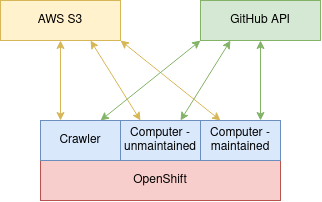
\includegraphics[scale=0.9]{chapters/chapter3/architecture.png}
    \caption{Data gathering architecture, Source: own}
    \label{fig:architecture}
\end{figure}

Figure \ref{fig:architecture} illustrates the data gathering process.
Three containers: \emph{crawler} \ref{sec:crawler}, \emph{computer - unmaintained} and \emph{computer - maintained} \ref{sec:computer} are running on the \emph{OpenShift} \ref{sec:openshift} platform.
Containers store and load data from the \emph{S3} storage \ref{sec:s3} and make calls to the \emph{GitHub API}.

\subsection{Tools used for data collection}

\subsubsection{Containers}
\label{sec:containers}

Containers contain a runtime environment which comprises the software application, its dependencies, libraries, binaries and configuration files.
The software application runs on the container and does not depend on the host environment except for the operating system.
A container can contain multiple apps and each app will have its own environment\footnote{See \url{https://www.techopedia.com/2/31967/trends/open-source/container-technology-the-next-big-thing}}.
Containerization thus provides a lightweight, isolated environment that makes apps easier to deploy and manage.

\begin{figure}
    \centering
    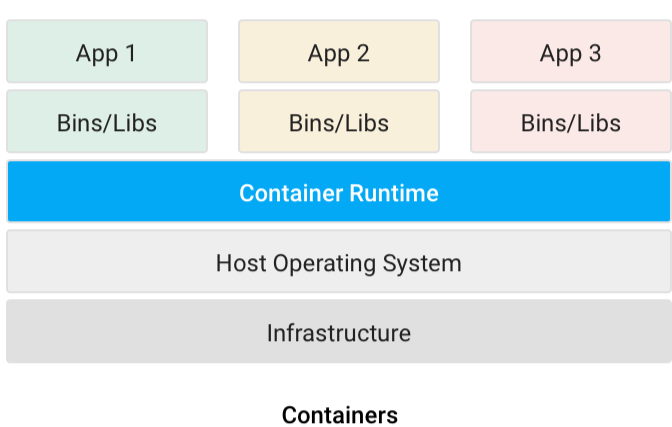
\includegraphics[scale=0.5]{chapters/chapter3/containerization.png}
    \caption{Container architecture\footnote{See \url{https://cloud.google.com/containers}}}
    \label{fig:container}
\end{figure}

Figure \ref{fig:container} shows the schema of a container architecture.
Applications \emph{App 1}, \emph{App 2} and \emph{App 3} are bundled with their dependencies and running on the \emph{container runtime}, software responsible for running containers.
\emph{Container runtime} runs on the host operating system which runs on the underlying infrastructure.

Running data collection components \ref{sec:crawler} and \ref{sec:computer} as containers has allowed me to take advantage of an Red Hat's OpenShift \ref{sec:openshift} cluster.

\subsubsection{OpenShift}
\label{sec:openshift}

Red Hat OpenShift\footnote{See \url{https://www.redhat.com/en/technologies/cloud-computing/openshift}} is an enterprise-ready Kubernetes\footnote{See \url{https://kubernetes.io/}} container platform.
It functions as a Platform-as-a-Service\footnote{See \url{https://www.oracle.com/cloud/what-is-paas/}} and a Container Orchestration\footnote{See \url{https://www.vmware.com/topics/glossary/content/container-orchestration}} Engine.

In the simplest of terms, it provides a platform for running and managing containers \ref{sec:containers}.
OpenShift is focused on a security on every level of a container stack, it also provides a huge set of other functionalities\footnote{See \url{https://www.openshift.com/}} including automated installation, upgrade, lifecycle manager and others.

\subsubsection{Amazon S3}
\label{sec:s3}

Data collection process is carried out by applications running as containers \ref{sec:containers}.
These applications generate data that need to be stored in the permanent storage outside of the containers.
\emph{Amazon S3}\footnote{See \url{https://aws.amazon.com/s3/}} provides such storage.

Amazon Simple Storage Service (Amazon S3) is an object storage service that offers industry-leading scalability, data availability, security, and performance.
Customers of all sizes and industries can use it to store and protect any amount of data for a range of use cases, such as data lakes, websites, mobile applications, backup and restore, archive, enterprise applications, IoT devices, and big data analytic\footnote{See \url{https://aws.amazon.com/s3/}}.

\subsection{Searching for suitable repositories}

\subsubsection{Filtering repositories}
\label{sec:filtering}

In the time of the study GitHub offers more than 38 million public repositories\footnote{See \url{https://github.com/search?q=is\%3Apublic\&ref=simplesearch}}.
Not all of them are suitable for this study, there are three minimal requirements repositories have to meet.

\begin{enumerate}
    \label{sec:suitable}
    \item \emph{Development time} \ref{feature:development_time} of more than 730 days (two years).
    Several features \ref{chap-3:features} require historical data.
    Idea behind is that estimating a longevity based on couple of weeks of development would be very inaccurate.
    % todo pidat citacie papierov kde brali featury z poslednych dvoch rokov vyvoja
    Several other studies used a similar time frame for evaluating repositories \cite{}.

    \item Repository contains a code in a programming language.
    Considerable portion of repositories do not contain files in a programming language.
    Examples are projects providing resource lists, CSS\footnote{See \url{https://developer.mozilla.org/en-US/docs/Learn/CSS/First\_steps/What\_is\_CSS}} templates or a content in some other markup or data type language.

    \item Project started a development using \emph{git} version control system.
    Some projects on GitHub were initially using some other version control\footnote{See \url{https://en.wikipedia.org/wiki/Template:Version\_control\_software}} and ported to \emph{git} in a later stage of the development.
    This devalues the data as the whole development process before the transition is squashed into a single or few commits, which do not realistically represent the full process from the start.

    A project is considered to be started outside of GitHub and then transitioned there later if more than 50\% of files were added in less than 20 commits.
    Same method is used in \cite{p:16}.

\end{enumerate}

Repositories satisfying previous criteria are considered suitable for the study.
Such projects are then divided into two categories.

\begin{enumerate}
\label{sec:(un)maintained}
    \item Unmaintained: there are three criteria necessary for unmaintained repositories:
        \begin{enumerate}
            \item Repository is archived\footnote{See \url{https://docs.github.com/en/github/creating-cloning-and-archiving-repositories/archiving-a-github-repository}}.
            Repository owners can archive their repositories to make it read-only and to let people know that the project will no longer be maintained.
            This is far better alternative to just deleting the repository, as users can still fork and use the archived projects.
            It would be very convenient for this study, if every unmaintained project was marked as archived.
            This is not the reality.
            While archiving projects that are no longer under active development is considered a good practice, it is not required.
            
            \item In some cases, repository owner puts the information about the end of development into the \emph{README} file.
            The crawler scans this file and marks a repository unmaintained if any of the following keywords is found: \emph{deprecated}, \emph{unmaintained}, \emph{no longer maintained}, \emph{no longer supported}, \emph{no longer under development}, \emph{not maintained}, \emph{not under development}, \emph{obsolete}, \emph{archived}.

            In some instances, such keyword can be used for some other purpose than to let the reader know that the project is no longer being developed.
            There are ... repositories classified as \emph{unmaintained} because of the found keyword in the README.
            For this reason, I manually checked all of such repositories to confirm if the repository was classified correctly.
            In the case of misclassification because of keyword used in some other context, said repository was reclassified correctly.
            Process was similar as in \cite{p:8}.

            \item Last criterion is that the last commit was submitted more then a year (104 weeks) ago.
            No activity for a year is a clear sign that the project's community is no longer continuing the development of the project.
        \end{enumerate}

    \item Maintained: suitable projects not considered unmaintained are viewed as maintained.
\end{enumerate}

Searching through repositories and their consecutive classification to not suitable/suitable and unmaintained/maintained is done by a \emph{crawler}.

\subsection{Developed applications}
\label{sec:applications}

\subsubsection{Repositories crawler}
\label{sec:crawler}

I created a crawler program to go through GitHub repositories and classifies \ref{sec:filtering} them.
Crawler goes through repositories in a random fashion.
The process is as follows:

\begin{enumerate}
    \item User selects a range of years for the crawler to search through.
    Repositories created within this time range will be considered for crawling.
    Input is added thru the configuration file \ref{sec:input}, the default search range and the one used for the study is years \emph{2009 - 2019}.
    Because of the \emph{suitability} requirement \ref{sec:suitable} of two years worth of historical data, the upper bound of this range is set to 2019.
    Repositories created after 2019 naturally do not have enough data to be fitting for the study.
    Lower bound is chosen arbitrarily.

    \item Time range is then transformed into an ID range.
    Repository IDs are represented as integers.
    Values of IDs of newly created repositories are higher than values of IDs of previously created repositories.
    This is convenient, as it can be exploited to make a random crawling of repositories easier.
    Transformation from a time range to an ID range is as follows:
    
    \begin{enumerate}
        \item Lower bound of an ID range is an ID of the first repository created in the year given by the lower bound of a time range.
        \item Upper bound of an ID range is an ID of the first repository created in the year given by the upper bound of a time range.
    \end{enumerate}

    \item Crawler that chooses an integer from the ID range with the uniform probability\footnote{Method used for this step of the process is \emph{random.randrange}, see \url{https://docs.python.org/3/library/random.html\#random.randrange}}.
    Not all IDs within the range still represent an existing repository, so the crawler needs to check the validity of the chosen integer.
    If the generated integer is a valid ID, process proceeds to the next step, if it is not, than it chooses another integer.

    % todo "vysiaca" referencia
    \item In the last step, the crawler classifies the repository \ref{sec:filtering} and saves the ID into the corresponding file.
\end{enumerate}

\subsection{Features computer}
\label{sec:computer}

Once the \emph{crawler} \ref{sec:crawler} gathers IDs of suitable repositories, another program, \emph{computer}, can compute the requested features of the repositories.
\emph{Computer} will go through the IDs collected by the \emph{crawler}.
For every ID, it will compute all of the implemented features specified in the \emph{configs/data\_gathering/features.yml} file \cite{repo}.

\subsection{Features of crawler and computer}

Although responsible for different tasks, both programs crawler and computer work in a very similar way.
They were both created with the same goals in mind.
Here are some notable features.

\subsubsection{Extensibility}

I proposed a set of features \ref{chap-3:features} to be used for the study.
New features can be added quickly:
they need to be implemented in the \emph{data\_gathering/repository\_data.py} and then referenced in the \emph{configs/data\_gathering/features.yml} file.

Extensibility is important, as it allows different users with different use cases to easily shape \emph{crawler} and \emph{computer} to better meet their specific needs.

\subsubsection{Scalability}

Project contains three \emph{Dockerfiles}\footnote{See \url{https://docs.docker.com/engine/reference/builder/}} for a \emph{crawler}, a \emph{computer} of unmaintained repositories and a \emph{computer} for maintained repositories.
These \emph{Dockerfiles} can be used to build containers \ref{sec:containers} which can be run on a container platform\footnote{See \url{https://en.wikipedia.org/wiki/OS-level_virtualization\#Implementations}}.
Users with sufficient resources can scale up a number of these containers and gather the data at a faster rate.

In the case of this project, applications were running as containers in the OpenShift cluster \ref{sec:openshift} provided by Red Hat\footnote{See \url{https://www.redhat.com/en}}.

\subsubsection{Flexibility}

Data gathering of on a sufficient scale takes up hundreds of hours.
The whole process does not need to finish in the single run.
Applications \emph{crawler} and \emph{computer} are build in such way that their computation can be terminated without the loss of previously computed data.

Both programs periodically and at the end of the execution serialize all of the computed data and upload them to the specified permanent storage.
At the beginning of the executions, both programs first check for the existing data in the permanent storage.
When preceding data is detected, applications will download them, unpack and then carry on with the computation.
Frequency of periodic saves and uploads of the data can be adjusted via a configuration file\footnote{See \url{https://github.com/samuelmacko/master\_thesis/blob/master/configs/data_gathering/gathering.yml}}.
Solution for the permanent storage used for this project is \emph{AWS S3} \ref{sec:s3}.

This alleviates the danger of losing potentially hours worth of computed data, in an event resulting in an application termination.
Containers can also be shut down, rebuild and re-run in order to update the application.

\subsubsection{Logging}

Both programs, \emph{crawler} and \emph{computer}, make use of detailed logging.
Log files are uploaded to the persistent storage with the other data.
This is useful in case of Pod\footnote{See \url{https://kubernetes.io/docs/concepts/workloads/pods/}} crashes which leave no Pod log file available.
Logs also inform about the progress of the data gathering and feature computation.

There are two levels of logging, NORMAL and DEBUG.
NORMAL level is mainly for displaying the progress, DEBUG on the other hand, shows more exhaustive progress information and possible errors.

\section{Dataset}

For the thesis, ... suitable \ref{sec:suitable} repositories were gathered.
Of these ... were classified as \emph{maintained} and the rest -- ... -- as \emph{unmaintained} \ref{sec:(un)maintained}.
\emph{Maintained} projects make only ...\% of all of the suitable repositories.
This small sample of all of the GitHub repositories indicates, that only a smaller fraction of them are under an active maintenance.

One of the conditions for the repository to be classified as \emph{unmaintained} is one of the selected keywords present in the \emph{README} file.


\section{Removing highly correlated features}

A dataset sample consists of 28 features \ref{chap-3:features}. 
I removed highly correlated features using \emph{Pearson correlation coefficient}\footnote{See \url{https://en.wikipedia.org/wiki/Pearson_correlation_coefficient}}.
Threshold for the removal is set to 90\%, sufficiently correlated -- and thus removed -- features are:

\begin{itemize}
    \item issues\_count\_open
    \item issues\_count\_closed
    \item releases\_count
    \item stargazers\_count
    \item wealth
\end{itemize}

Correlation heatmap can be seen in the figure \ref{fig:heatmap}.
Final number of features is then 23.

\begin{figure}
    \centering
    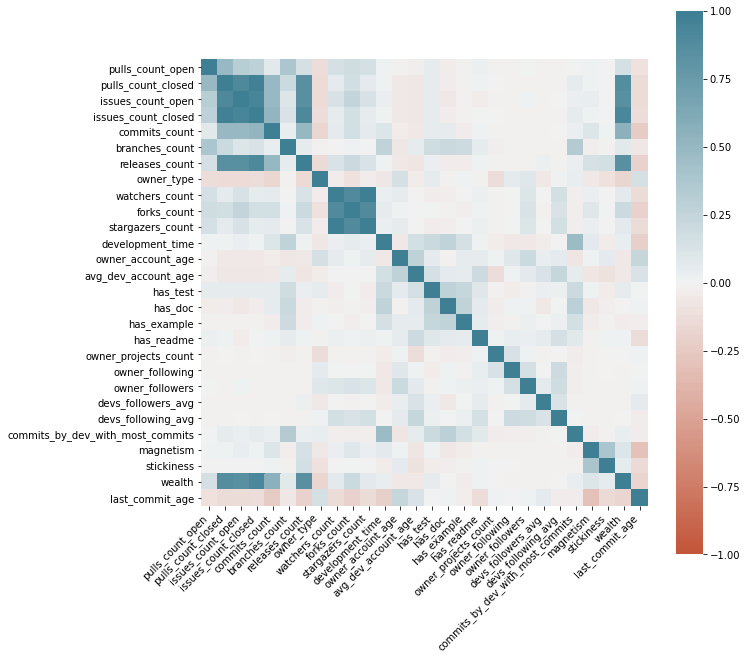
\includegraphics[scale=0.5]{chapters/chapter3/corr-heatmap.png}
    \caption{Correlation heatmap}
    \label{fig:heatmap}
\end{figure}

% todo nejake grafy descriptive statistics
% mean, standard deviation, skewness, quartiles niektorych featur
% kolko ma readme, testy a take veci
% vizualizacia: boxploty pre mean, variance, ...
% "podozrive" featury na korelaciu overit aj statistickymi testami a potom nepouzivat v datasete

\section{Dataset preprocessing}

Features of the dataset have data of both types, numeric and categorical.
Integer and float features all have different means and ranges.
For a dataset to be usable as an input for used machine learning algorithms \ref{sec:models}, the data needs to be processed.

Numeric features are measured in different ranges and in different units (days, contributors, commits, etc.).
Such input data would not produce a valid results, as features with higher range values would dominate over features with values in lower ranges.
Several distance-based machine learning models would attribute higher weight to features with a higher magnitude and thus biasing the result.
To prevent this problem, feature scaling solution \emph{StandardScaler}\footnote{See \url{https://scikit-learn.org/stable/modules/generated/sklearn.preprocessing.StandardScaler.html}} was used.
\emph{StandardScaler} subtracts the mean value from the feature and then divides the result by the feature standard deviation.
This process produces data that have mean value of 0 and standard deviation of 1.

Apart from the numeric features, dataset also contains nominal categorical features.
While these features are encoded as integers, there is no particular order between categories.
Using these integers as input would skew the models as categories with higher value integer would arbitrarily be assigned a higher weight.
Encoding such features is done by \emph{OneHotEncoder}\footnote{See \url{https://scikit-learn.org/stable/modules/generated/sklearn.preprocessing.OneHotEncoder.html}}, it transforms a categorical feature with \emph{n} possible values into \emph{n} binary features.

Whole preprocessing process can be seen in the figure \ref{fig:preprocessing}.
Maintained repositories are not used for the training nor for the evaluation, only for the computation of the centroid.
The centroid is needed for the labeling \ref{sec:labeling} of projects classified as unmaintained.

These unmaintained projects are split to two sets, one used for training and the other used for testing.
Training set contains 80\% of all of the unmaintained repositories.
The rest, 20\%, is used for testing.
Features of these sets are preprocessed separately.
This is because \emph{StandardScaler} uses mean and standard deviation of the samples for its computation.
If both -- test and training -- sets were preprocessed together, information from the training set would leak\footnote{See \url{https://machinelearningmastery.com/data-leakage-machine-learning/}} into the test set, which is undesirable.

\begin{figure}
    \centering
    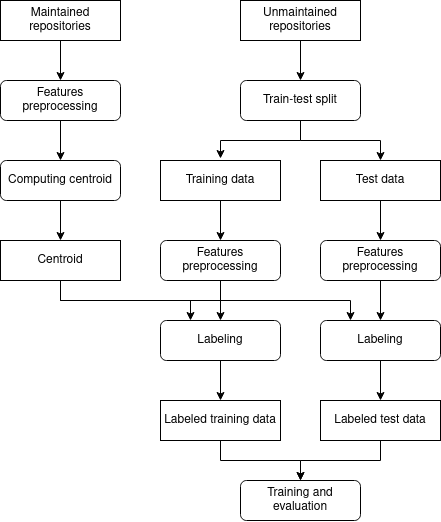
\includegraphics[scale=0.8]{chapters/chapter3/preprocessing.png}
    \caption{Scheme of preprocessing}
    \label{fig:preprocessing}
\end{figure}

\section{Samples labeling}
\label{sec:labeling}

Classification models are trained in a supervised manner, this means that the training data need to be labeled.
Labeling process is as follows:

\begin{enumerate}
    \item Gather a sufficient quantity of suitable repositories \ref{sec:filtering}.

    \item Cluster \emph{maintained} repositories and find their centroid using a KMeans algorithm\footnote{See \url{https://scikit-learn.org/stable/modules/generated/sklearn.cluster.KMeans.html}}.
    Centroid is central vector, which may not necessarily be a member of the data set.
    The centroid can be thought of as the multi-dimensional average of the cluster.

    \item Compute an \emph{l2}\footnote{See \url{https://scikit-learn.org/stable/modules/generated/sklearn.metrics.pairwise.euclidean_distances.html}} (Euclidean) distance of every \emph{unmaintained} repository from the \emph{maintained} repository cluster centroid.
    
    \item Create a subset of \emph{unmaintained} repositories with outliers removed.
    Outliers are determined using \emph{Interquartile range} approach\footnote{See \url{https://www.statology.org/find-outliers-with-iqr/}} computed on the Euclidean distances of repositories from the centroid.

    \item Based on this subset, 10 equally sized bins are created.

    \item Label all repositories based on the bin they belong to.
    Repositories with the distance greater than the limit of the last bin are put into that last bin, and repositories smaller than the limit of the smallest bin are put into the smallest one.
\end{enumerate}

Labeled train and test data are then used in the training and evaluation process \ref{sec:training_evaluation}.
% todo hodit histogram lablov

\section{Training and evaluation}
\label{sec:training_evaluation}

Four machine learning algorithms were tested for the best result, these are:

\begin{enumerate}
\label{sec:models}
    \item RandomForest\footnote{See \url{https://scikit-learn.org/stable/modules/generated/sklearn.ensemble.RandomForestClassifier.html}}
    \item SVC\footnote{See \url{https://scikit-learn.org/stable/modules/generated/sklearn.svm.SVC.html}}
    \item kNN\footnote{See \url{https://scikit-learn.org/stable/modules/generated/sklearn.neighbors.KNeighborsClassifier.html}}
    \item MLP\footnote{See \url{https://scikit-learn.org/stable/modules/generated/sklearn.neural_network.MLPClassifier.html}}
\end{enumerate}

Best set of hyper-parameters for models \ref{sec:models} were tuned using \emph{grid search}\footnote{See \url{https://scikit-learn.org/stable/modules/generated/sklearn.model_selection.GridSearchCV.html\#sklearn.model_selection.GridSearchCV}}.
Using \emph{grid search} technique, every possible combination of pre-defined hyper-parameters is tried and evaluated in order to find the set with the best performance.
Parameter grids used in the thesis can be seen in the tables \ref{tab:grid-rf}, \ref{tab:grid-knn}, \ref{tab:grid-svm} and \ref{tab:grid-mlp}.

Models are evaluated using 5-fold \emph{cross validation}\footnote{See \url{https://en.wikipedia.org/wiki/Cross-validation_(statistics)}}.
Two scores were used for evaluating quality of model's predictions.

\begin{enumerate}
    \item Accuracy - simple fraction of correct predictions and all predictions.

    \item Custom accuracy score with deviation:
    Very similar to accuracy score, but prediction label of one more or one less than the true label is still considered as a correct prediction.
    For example, true label is 7.
    If the model predicts 6, 7, or 8, all of these are considered a correct prediction.
    Number of correct predictions is then divided by the number of all predictions as usual.
    
    I added this score to compute accuracy with small deviation, if the user cares accepts a small error in predictions.
    
\end{enumerate}

% todo doplnint
\begin{table}
  \caption{Parameters grid for RandomForest}
  \label{tab:grid-rf}
  \begin{tabular}{|c|c|}
    \toprule
    Hyper-parameter & Values \\
    \midrule
    criterion & gini, entropy \\
    \bottomrule
  \end{tabular}
\end{table}

% todo doplnint
\begin{table}
  \caption{Parameters grid for SVM}
  \label{tab:grid-svm}
  \begin{tabular}{|c|c|}
    \toprule
    Hyper-parameter & Values \\
    \midrule
    criterion & gini, entropy \\
    \bottomrule
  \end{tabular}
\end{table}

% todo doplnint
\begin{table}
  \caption{Parameters grid for kNN}
  \label{tab:grid-knn}
  \begin{tabular}{|c|c|}
    \toprule
    Hyper-parameter & Values \\
    \midrule
    criterion & gini, entropy \\
    \bottomrule
  \end{tabular}
\end{table}

% todo doplnint
\begin{table}
  \caption{Parameters grid for MLP}
  \label{tab:grid-mlp}
  \begin{tabular}{|c|c|}
    \toprule
    Hyper-parameter & Values \\
    \midrule
    criterion & gini, entropy \\
    \bottomrule
  \end{tabular}
\end{table}


\chapter{Results}
\label{chap-4:results}


\chapter{Summary}
\label{chap-5:summary}


% \begin{description}
%   \item[Description list]
%     A list of terms with a description of each term
% \end{description}

% The spacing of these lists is geared towards paragraphs of text.
% For lists of words and phrases, the \textsf{paralist} package
% offers commands
% \begin{compactitem}
%   \item that
%   \begin{compactitem}
%     \item are
%     \begin{compactitem}
%       \item better
%       \begin{compactitem}
%         \item suited
%       \end{compactitem}
%     \end{compactitem}
%   \end{compactitem}
% \end{compactitem}
% \begin{compactenum}
%   \item to
%   \begin{compactenum}
%     \item this
%     \begin{compactenum}
%       \item kind of
%       \begin{compactenum}
%         \item content.
%       \end{compactenum}
%     \end{compactenum}
%   \end{compactenum}
% \end{compactenum}

% The \textsf{amsthm} package provides the commands necessary for the
% typesetting of mathematical definitions, theorems, lemmas and
% proofs.

% %% We will define several mathematical sectioning commands.
% \newtheorem{theorem}{Theorem}[section] %% The numbering of theorems
%                               %% will be reset after each section.
% \newtheorem{lemma}[theorem]{Lemma}         %% The numbering of lemmas
% \newtheorem{corollary}[theorem]{Corollary} %% and corollaries will
%                               %% share the counter with theorems.
% \theoremstyle{definition}
% \newtheorem{definition}{Definition}
% \theoremstyle{remark}
% \newtheorem*{remark}{Remark}

% \begin{theorem}
%   This is a theorem that offers a profound insight into the
%   mathematical sectioning commands.
% \end{theorem}
% \begin{theorem}[Another theorem]
%   This is another theorem. Unlike the first one, this theorem has
%   been endowed with a name.
% \end{theorem}
% \begin{lemma}
%   Let us suppose that $x^2+y^2=z^2$. Then
%   \begin{equation}
%     \biggl\langle u\biggm|\sum_{i=1}^nF(e_i,v)e_i\biggr\rangle
%     =F\biggl(\sum_{i=1}^n\langle e_i|u\rangle e_i,v\biggr).
%   \end{equation}
% \end{lemma}
% \begin{proof}
%   $\nabla^2 f(x,y)=\frac{\partial^2f}{\partial x^2}+
%   \frac{\partial^2f}{\partial y^2}$.
% \end{proof}
% \begin{corollary}
%   This is a corollary.
% \end{corollary}
% \begin{remark}
%   This is a remark.
% \end{remark}

% \begin{figure}
%   \begin{center}
%     \begin{minipage}{.66\textwidth}
%       
\includegraphics[width=\textwidth]{fithesis/logo/mu/fithesis-base.pdf}
%     \end{minipage}
%     \begin{minipage}{.33\textwidth}
%       
\includegraphics[width=\textwidth]{fithesis/logo/mu/fithesis-base.pdf} \\
%       
\includegraphics[width=\textwidth]{fithesis/logo/mu/fithesis-base.pdf}
%     \end{minipage}
%   \end{center}
%   \caption{The logo of the Masaryk University at $\frac23$ and
%     $\frac13$ of text width}
%   \label{fig:mulogo2}
% \end{figure}

% \begin{table}
%   \begin{tabularx}{\textwidth}{lllX}
%     \toprule
%     Day & Min Temp & Max Temp & Summary \\
%     \midrule
%     Monday & $13^{\circ}\mathrm{C}$ & $21^\circ\mathrm{C}$ & A
%     clear day with low wind and no adverse current advisories. \\
%     Tuesday & $11^{\circ}\mathrm{C}$ & $17^\circ\mathrm{C}$ & A
%     trough of low pressure will come from the northwest. \\
%     Wednesday & $10^{\circ}\mathrm{C}$ &
%     $21^\circ\mathrm{C}$ & Rain will spread to all parts during the
%     morning. \\
%     \bottomrule
%   \end{tabularx}
%   \caption{A weather forecast}
%   \label{tab:weather}
% \end{table}

% \chapter{Mathematical equations}
% \label{chap:matheq}
% \TeX{} comes pre-packed with the ability to typeset inline
% equations, such as $\mathrm{e}^{ix}=\cos x+i\sin x$, and display
% equations, such as \[
%   \mathbf{A}^{-1} = \begin{bmatrix}
%   a & b \\ c & d \\
%   \end{bmatrix}^{-1} =
%   \frac{1}{\det(\mathbf{A})} \begin{bmatrix}
%   \,\,\,d & \!\!-b \\ -c & \,a \\
%   \end{bmatrix} =
%   \frac{1}{ad - bc} \begin{bmatrix}
%   \,\,\,d & \!\!-b \\ -c & \,a \\
%   \end{bmatrix}.
% \] \LaTeX{} defines the automatically numbered \texttt{equation}
% environment:
% \begin{equation}
%   \gamma Px = PAx = PAP^{-1}Px.
% \end{equation}
% The package \textsf{amsmath} provides several additional
% environments that can be used to typeset complex equations:
% \begin{enumerate}
%   \item An equation can be spread over multiple lines using the
%     \texttt{multline} environment:
%     \begin{multline}
%       a + b + c + d + e + f + b + c + d + e + f + b + c + d + e +
% f \\
%       + f + g + h + i + j + k + l + m + n + o + p + q
%     \end{multline}

%   \item Several aligned equations can be typeset using the
%     \texttt{align} environment:
%     \begin{align}
%               a + b &= c + d     \\
%                   u &= v + w + x \\[1ex]
%       i + j + k + l &= m
%     \end{align}

%   \item The \texttt{alignat} environment is similar to
%     \texttt{align}, but it doesn't insert horizontal spaces between
%     the individual columns:
%     \begin{alignat}{2}
%       a + b + c &+ d       &   &= 0 \\
%               e &+ f + g   &   &= 5
%     \end{alignat}

%   \item Much like chapter, sections, tables, figures, or list
%     items, equations -- such as \eqref{eq:first} and
%     \eqref{eq:mine} -- can also be labeled and referenced:
%     \begin{alignat}{4}
%       b_{11}x_1 &+ b_{12}x_2  &  &+ b_{13}x_3  &  &             &
%         &= y_1,                   \label{eq:first} \\
%       b_{21}x_1 &+ b_{22}x_2  &  &             &  &+ b_{24}x_4  &
%         &= y_2. \tag{My equation} \label{eq:mine}
%     \end{alignat}

%   \item The \texttt{gather} environment makes it possible to
%     typeset several equations without any alignment:
%     \begin{gather}
%       \psi = \psi\psi, \\
%       \eta = \eta\eta\eta\eta\eta\eta, \\
%       \theta = \theta.
%     \end{gather}

%   \item Several cases can be typeset using the \texttt{cases}
%     environment:
%     \begin{equation}
%       |y| = \begin{cases}
%         \phantom-y & \text{if }z\geq0, \\
%                 -y & \text{otherwise}.
%       \end{cases}
%     \end{equation}
% \end{enumerate}
% For the complete list of environments and commands, consult the
% \textsf{amsmath} package manual\footnote{
%   See \url{http://mirrors.ctan.org/macros/latex/required/amslatex/math/amsldoc.pdf}.
%   The \texttt{\textbackslash url} command is provided by the
%   package \textsf{url}.
% }.

\printbibliography[heading=bibintoc] %% Print the bibliography.

\makeatletter\thesis@blocks@clear\makeatother
\phantomsection %% Print the index and insert it into the
\addcontentsline{toc}{chapter}{\indexname} %% table of contents.
\printindex

\appendix %% Start the appendices.
\chapter{An appendix}
Here you can insert the appendices of your thesis.

\end{document}
